
\documentclass[ms.tex]{subfiles}
\begin{document}

\section{Results}
\label{sec:results}

\subsection{Evolution of a Fiducial Model}
\label{sec:results:fiducial}

% fig 5
\begin{figure*}
\centering
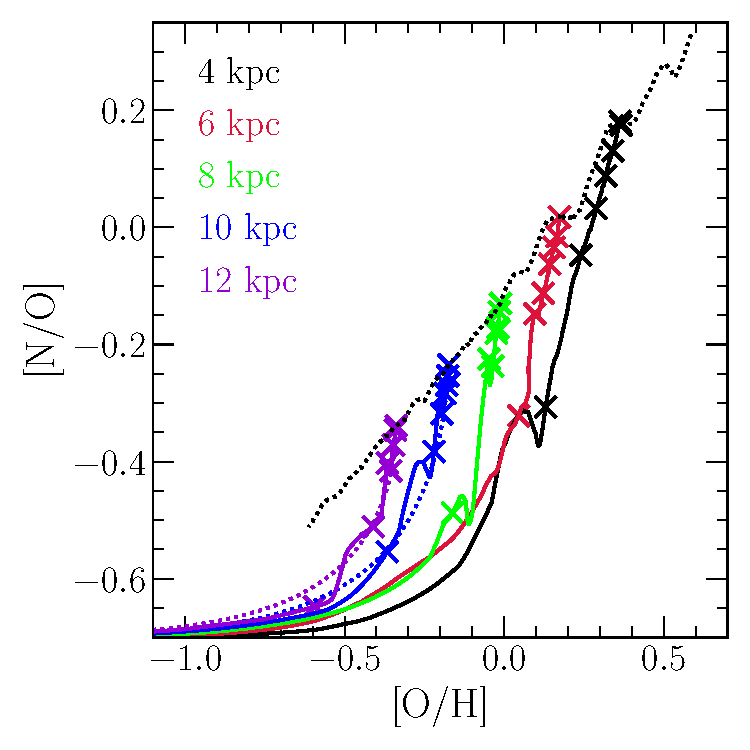
\includegraphics[scale = 0.63]{no_oh_superposition.pdf}
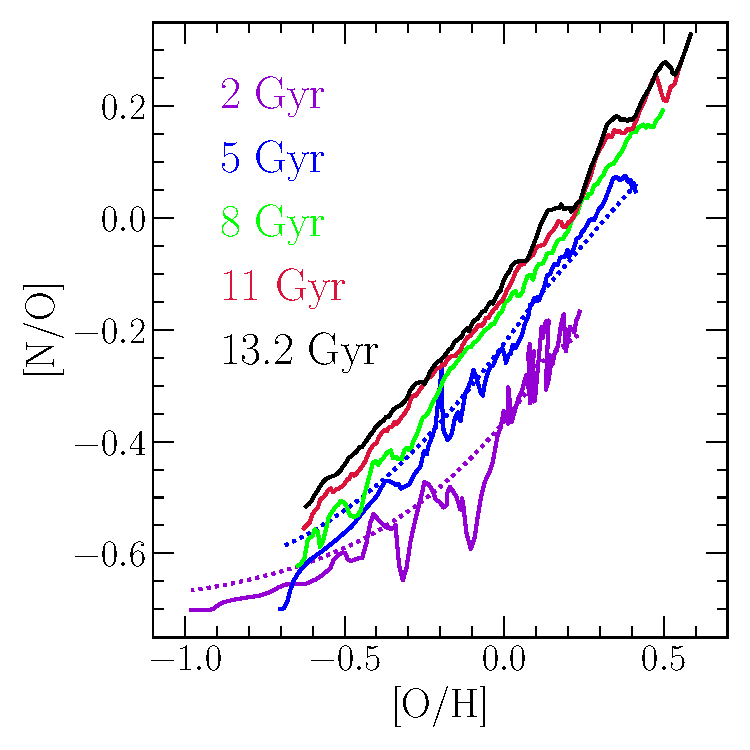
\includegraphics[scale = 0.63]{no_oh_timeevol.pdf}
\caption{
\textbf{Left}: The gas-phase~\ohno~relation parameterized by time at
fixed radius (solid coloured lines) in the fiducial model. X's denote the
abunadnces at~$T = 2$, 4, 6, 8, 10, 12, and 13.2 Gyr (the present day) at all
radii.
The dotted black line is the same as the solid black line in the right panel.
Coloured dotted lines mark the evolution of our model at~$\rgal = 10$ and 12
kpc when stellar migration is neglected (i.e. the ``post-processing'' migration
model from~\citealp{Johnson2021}).
\textbf{Right}: The gas-phase~\ohno~relation parameterized by radius at
various snapshots (solid coloured lines) in our fiducial model.
Similar to the left panel, coloured dotted lines denote the resulting relation
at~$T = 2$ and 5 Gyr when we neglect stellar migration.
}
\label{fig:no_oh_timeevol}
\end{figure*}

Our fiducial model adopts~$\ycc{N} = 3.6\times10^{-4}$ and our linear AGB star
yield model with~$\xi = 9\times10^{-4}$ (see equation~\ref{eq:linear_yield})
along with the O and Fe yields of~\citet[][see discussion
in~\S~\ref{sec:yields:ccsne}]{Johnson2021}.
Although we presented this model in comparison to the~\cristallo~yields with
$\xi = 3\times10^{-4}$ in Fig.~\ref{fig:agb_yield_models}, we find that a
renormalization of this model is necessary to reproduce the~\ohno~relation as
observed; we discuss this point further in~\S~\ref{sec:results:yields}.
To demonstrate the impact of stellar migration on N enrichment rates, we make
use of the diffusion migration model in this section (see discussion
in~\S~\ref{sec:multizone}).
\par
In the left panel of Fig.~\ref{fig:no_oh_timeevol}, we plot the evolution of N
and O abundances in the gas phase at five different Galactocentric radii.
At early times,~\oh~is low and~\no~reflects the ratio of the CCSN yields
(\no\subcc~$\approx -0.7$).
Consequently, the tracks in each ring are similar.
Once lower mass stars begin to evolve through an AGB phase, they enrich the
interstellar medium (ISM) with N but negligible amounts of O, increasing~\no.
At this point, the tracks in each ring separate from one another.
This separation is a consequence of the metallicity gradient in~\oh~being
established early in the Galaxy's evolution.
Being an element produced primarily by CCSNe on short delay times, O reaches
an equilibrium abundance before elements produced by significantly delayed
nucleosynthetic sources~\citep{Weinberg2017}.
The ISM achieves equilibrium in O soon after AGB stars begin producing N,
after which~\no~continues to increase at an approximately fixed~\oh~at all
radii (see also Fig.~\ref{fig:nh_feh_vs_lookback} and associated discussion
in~\S~\ref{sec:results:vincenzo_comp}).
The N and O abundances of the Galaxy in the past therefore differ from that
which would be derived observationally by taking their values at the present
day from all rings (shown by the black dotted line, see discussion below).
% The relation that would be derived observationally for this model by taking the
% N and O abundances at the present day from all rings (shown by the
% dotted black line, see discussion below) does not reflect the N and O
% abundances of the Galaxy in the past.
This contests the popular assumption that the~\ohno~relation in Milky Way-mass
galaxies arises as an evolutionary sequence, instead suggesting a superposition
of endpoints like that previously suggested for low [$\alpha$/Fe] disc stars
\citep[e.g.][]{Schoenrich2009, Nidever2014, Buck2020, Sharma2021}.
\par
Because there is a delay between a stellar population's formation and N
production from its AGB stars ($\sim$250 Myr in this model; see Fig.
\ref{fig:ssp}), stellar migration can in principle occur within this time
interval.
Although the bulk of migration occurs on longer timescales, this characteristic
delay is comparable to the dynamical time of the Milky Way and is thus adequate
for kinematic heating to at least begin.
As a consequence, there may be a slight deficit or surplus of N-producing AGB
stars in a given ring at some time induced by stellar migration.
These tracks can thus move vertically in this plane in response to AGB stars
moving between rings as the Galaxy evolves, entirely independent of the SFH and
the nucleosynthetic yields of stars than formed at a given radius and time.
We demonstrate this effect by comparing the solid blue and purple lines to
their dotted counterparts.
These are the tracks we compute using the post-processing migration model,
which neglects the impact of migration on enrichment rates (see discussion
in~\S~\ref{sec:multizone}).
\par
In the right panel of Fig.~\ref{fig:no_oh_timeevol}, we plot the
gas-phase~\ohno~relation predicted by the model at various snapshots.
To obtain this, we simply take the N and O abundances in the ISM at a given
output time for each~$\delta\rgal = 100$ pc ring at~$\rgal > 2$ kpc and plot
them as a line.
The relation is generally time-independent at~$T \gtrsim 5$ Gyr.
Although there is some slight evolution toward higher~\no, the total change
in~\no~over this time interval is well within the intrinsic scatter derived
observationally (see Fig.~\ref{fig:no_oh_observed}).
Even at~$T = 2$ Gyr at a redshift of~$z \approx 2.6$ (when the universe was
2.5 Gyr old, see discussion in~\S~\ref{sec:multizone}),~\no~at
fixed~\oh~is only~$\sim$0.2 dex lower than its value at the present day.
Especially when considering the intrinsic scatter that would arise if we were
to consider models with, e.g., different SFHs, this supports previous
arguments that the redshift evolution of the~\ohno~relation is at most
minimal~\citep{Vincenzo2018, HaydenPawson2021}.
\par
We again demonstrate the impact of stellar migration in the right panel of
Fig.~\ref{fig:no_oh_predictions} by comparing the blue and purple solid lines
to their dotted counterparts, which quantify the relation using the
post-processing migration model.
This indicates that the complex features seen in the relation at all times are
a consequence of migration as discussed above.
The mechanism by which stellar migration imposes these features in
the~\ohno~plane is qualitatively similar to what~\citet{Johnson2021} find for
SN Ia production of Fe (see discussion in their~\S\S~3.1 and 3.4).
They found that the SN Ia rate in this model can vary by as much as a factor of
$\sim$3 at large radii ($\rgal \gtrsim 9$ kpc).
When a deficit or surplus of SN Ia events is sustained for timescales
comparable to the depletion time of the local ISM, the gas-phase abundance of
Fe increases or decreases accordingly.
As a consequence, some of the stellar populations that form during these
events are Fe-poor enough to present as young stars ($\lesssim$ 6 Gyr) with
significantly super-solar [$\alpha$/Fe] ratios.
Stars with these ages and chemical compositions have indeed been observed in
the solar neighbourhood with APOGEE~\citep{Chiappini2015, Martig2015,
Martig2016, Warfield2021}.
Although a substantial portion of the observed stars appear to have undergone
mass transfer from a binary companion, allowing them to masquerade as younger
objects~\citep{Jofre2016, Yong2016, Izzard2018, SilvaAguirre2018, Miglio2021},
some exhibit [C/N] ratios consistent with truly young ages~\citep{Hekker2019}.
\citet{Johnson2021} argue that the impact of stellar migration on enrichment
rates is responsible for this intrinsically young sub-component (see
discussion in their~\S~3.4).
% Stars with these ages and chemical compositions have indeed been observed with
% APOGEE~\citep{Chiappini2015, Martig2015, Martig2016, Jofre2016, Yong2016,
% Izzard2018, SilvaAguirre2018, Miglio2021}, and~\citet{Johnson2021} argue that
% an intrinsically young sub-component of this population~\citep{Hekker2019}
% could arise as a consequence of the impact of migration on enrichment rates
% (see discussion in their~\S~3.4).
In the case of N, the effect is much smaller ($\lesssim$ 0.1 dex in~\no),
but Fig.~\ref{fig:no_oh_timeevol} suggests there are some instances at early
times where the effect is more substantial.
This arises because our model predicts N yields to be ejected from stellar
populations~$\sim$5 times faster than Fe (even faster in our alternate yield
models with larger contributions from high mass AGB stars; see Fig.
\ref{fig:ssp} and discussion in~\S~\ref{sec:yields:imf_agb}).
Consequently, there is much less time for stellar migration to occur within the
timescale of N production than there is within the timescale of Fe production.
This underscores the argument from~\citet{Johnson2021} that the impact of
stellar migration on enrichment rates is more substantial for elements
produced on longer characteristic delay times.


\subsection{Comparison to Observed Gas-Phase Trends}
\label{sec:results:yields}

% fig 6
\begin{figure*}
\centering
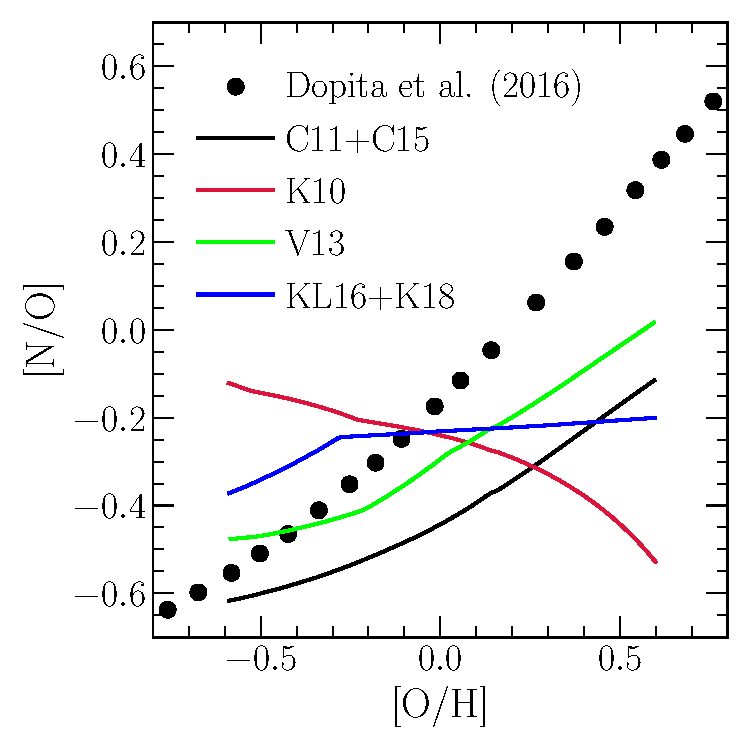
\includegraphics[scale = 0.45]{no_oh_predictions_unmodified.pdf}
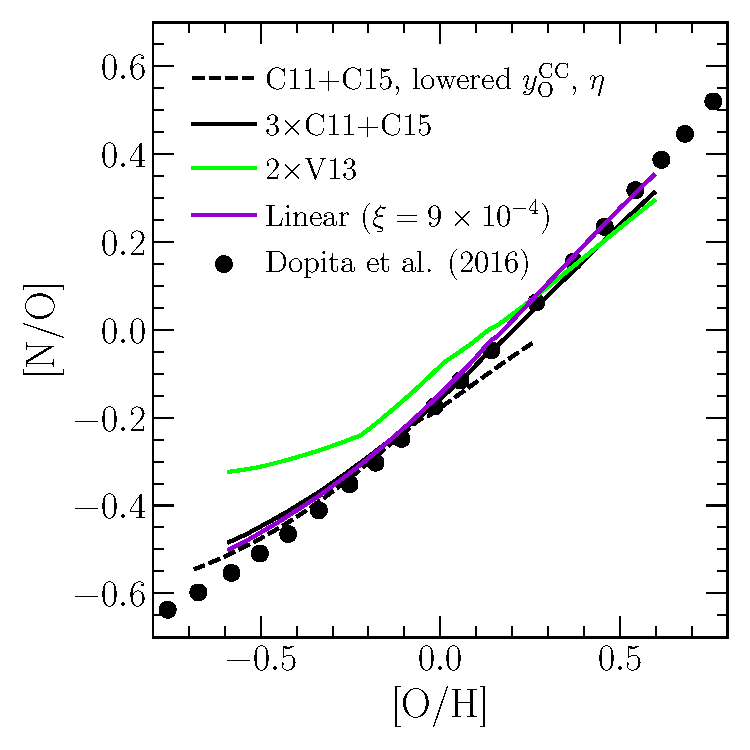
\includegraphics[scale = 0.45]{no_oh_predictions.pdf}
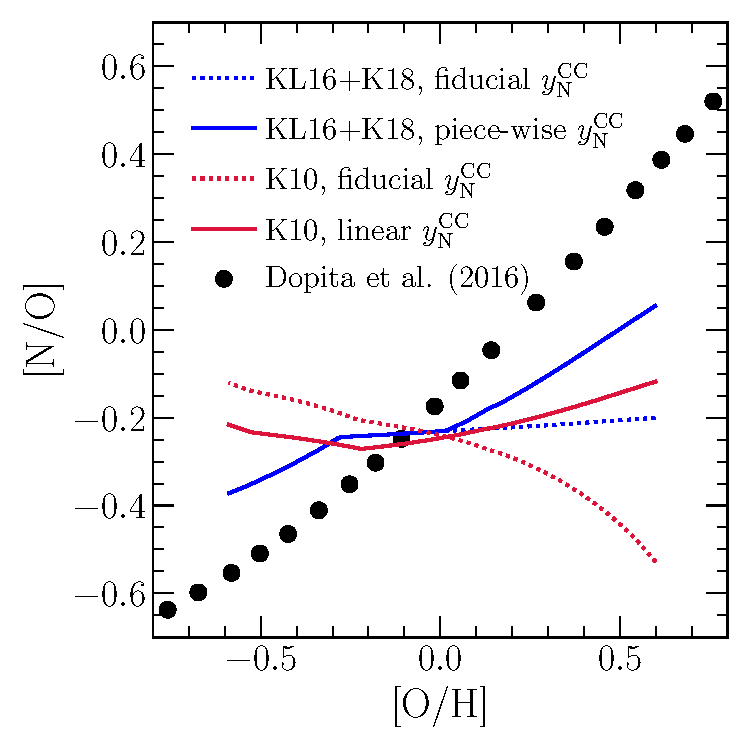
\includegraphics[scale = 0.45]{no_oh_predictions_karakas.pdf}
\caption{
\textbf{Left}: The present-day gas-phase~\ohno~relation predicted by our
model with each of the four yield models based on stellar evolution models
discussed in~\S~\ref{sec:yields:agb}, colour-coded according to the legend.
We include the~\citet{Dopita2016} measurements of this relation for local stars
and HII regions (duplicated from Fig.~\ref{fig:no_oh_observed}) as the
observational benchmark.
\textbf{Middle}: The same as the left panel, but for a case where we
artificially amplify the~\cristallo~yields by a factor of 3 and
the~\ventura~yields by a factor of 2.
We include our linear model as well, but with the slope amplified from
$\xi = 3\times10^{-4}$ as shown in Fig.~\ref{fig:agb_yield_models} to
$\xi = 9\times10^{-4}$ since it is also based on the~\cristallo~yields.
\textbf{Right}: The same as the left panel, but comparing the predictions made
by the~\karakasten~and~\karakas~yields with our fiducial value of
$y_\text{N}^\text{CC}$ (dotted lines, same as left-hand panel) to those with
alternate forms of~$y_\text{N}^\text{CC}$ (solid lines; see discussion in~\S
\ref{sec:results:yields}).
We show all predictions with ``post-processing'' migration model (see
discussion in~\S~\ref{sec:multizone}).
}
\label{fig:no_oh_predictions}
\end{figure*}

We use the~\citet{Dopita2016} measurements as our observational benchmark.
They are a good representation of many results for gas-phase N and O abundances
(see Fig.~\ref{fig:no_oh_observed}), and they agree well with APOGEE stellar
trends~\citep{Vincenzo2021}.
To make the comparison between different yield models more clear, we neglect
the impact of stellar migration on enrichment rates and make use of the
post-processing migration model in this section (see discussion
in~\S~\ref{sec:multizone}).
\par
In the left panel of Fig.~\ref{fig:no_oh_predictions}, we compare our model
predictions with each of the AGB star yield tables predicted from stellar
evolution models (see Fig.~\ref{fig:agb_yield_models} and discussion
in~\S~\ref{sec:yields:agb}).
Because our linear model (see equation~\ref{eq:linear_yield}) with a slope of
$\xi = 3\times10^{-4}$ is based on the~\cristallo~yields, the two make similar
predictions.
With no changes to the~\citet{Johnson2021} parameterization of the model, all
four AGB star yield tables fail to reproduce the~\ohno~relation as observed.
The~\cristallo~and~\ventura~yields are able to reproduce the qualitative trend,
but with an incorrect normalization.
The~\karakasten~and~\karakas~yields, on the other hand, fail to reproduce
the steadily sloped increase of~\no~with~\oh.
The inverse dependence of~\no~with~\oh~predicted by the~\karakasten~AGB star
yields can be understood by the interaction between TDU and HBB (see discussion
in~\S~\ref{sec:yields:agb}).
Both effects are stronger at low metallicity, and since all of
the~\karakasten~stars experiencing HBB also experience TDU (see their Table 1),
such a result is unsurprising.
This is also true for the~\karakas~yields, but that model predicts a
relatively flat~\ohno~relation because of updated model inputs regarding
opacity and mass loss and the impact this has on~\Nfourteen~yields (see
discussion in~\S~\ref{sec:yields:agb}).
\par
In order to successfully reproduce the observations with
the~\cristallo~and~\ventura~yields, we find that we must artificially amplify
them by factors of~$\sim$3 and~$\sim$2, respectively.
Having originally compared our linear model to the~\cristallo~yields in
Fig.~\ref{fig:agb_yield_models} with a slope of~$\xi = 3\times10^{-4}$, we
amplify this value by a factor of 3 here as well.
We illustrate the results of these modified yield models in the middle panel
of Fig.~\ref{fig:no_oh_predictions}.
Although the~\ventura~model predicts an~\ohno~relation that is slightly
shallower than the~\citet{Dopita2016} measurements, the predictions are
reasonably within the scatter seen in Fig.~\ref{fig:no_oh_observed}.
Rather than artificially amplifying the~\cristallo~and~\ventura~yields, we also
find good agreement with the observed relation if we lower both our SN yields
and our outflow mass loading factor~$\eta$ as a function of~\rgal~by similar
factors from their values in~\citet{Johnson2021}.
These parameters, which approximately determine the equilibrium abundance in a
one-zone model~\citep{Weinberg2017}, are tuned to reproduce a metallicity
gradient in the disc that resembles that observed for the Milky Way (see
discussion in~\S~2.4 of~\citealp{Johnson2021}).
However, since the yield and the outflow are simply source and sink terms in
computing enrichment rates, the model makes similar predictions when both are
raised or lowered by the same factor.
We demonstrate this point in the middle panel of Fig.
\ref{fig:no_oh_predictions} with the black dashed line for the~\cristallo~model
with both~\ycc{O}~and~$\eta$ each lowered by a factor of 3.
This model spans a different range in~\oh~because the relation between~\ycc{O},
$\eta$, and the equilibrium abundance is only approximately one-to-one, but the
predictions also exhibit good agreement with the~\citet{Dopita2016}
measurements.
\par
Lowering our SN yields by a factor of~$2 - 3$ is plausible if a substantial
fraction of massive stars collapse directly to black holes as opposed to
exploding as SNe at the ends of their lives.
Our IMF-averaged massive star yields (see discussion in~\S
\ref{sec:yields:ccsne}) are based on a~\citet{Kroupa2001} IMF combined with SN
nucleosynthesis models in which most~$M > 8~\msun$ stars explode as a CCSN
\cite[e.g.][]{Woosley1995, Chieffi2004, Chieffi2013, Limongi2018, Nomoto2013},
but recent results contest the validity of this assumption.
The criteria for massive star explosions and which stars of what masses end
their lives in ``failed supernovae'' has been a recent topic of interest from
both theoretical~\citep[e.g.][]{Pejcha2015, Sukhbold2016, Ertl2016} and
observational perspectives (e.g.~\citealp*{Gerke2015};~\citealp{Adams2017,
Basinger2021}).
Although there is presently no combination of a SN nucleosynthesis model with
a physically motivated black hole landscape is able to reproduce the observed
abundance patterns~\citep{Griffith2021a}, black hole formation still lowers
SN yields by simply not ejecting massive star envelopes to the ISM.
With~\vice's~\texttt{vice.yields.ccsne.fractional} function, designed to
calculate values of~\ycc{X}~for various elements (see discussion
in~\S~\ref{sec:yields:ccsne} here and in~\S~4 of~\citealp{Griffith2021a}), we
indeed find a value of~$\ycc{O} = 0.0056$ using the W18 explosion model from
\citet{Sukhbold2016} compared to our fiducial value of~$\ycc{O} = 0.015$.
\par
Alternatively,~\citet{Vincenzo2016a} are able to reproduce the~\ohno~relation
in chemical evolution models with the~\ventura~yields by implementing a
differential wind in which outflows remove O but not N from the star forming
gas reservoir.
Because the enrichment rates are the same as in our models with lowered
yields, we find similar results if we simply add a portion of the SN products
(both CCSN and SN Ia) directly to the outflow while still lowering~$\eta$ at
all radii.
If SNe are the sources of outflow-driving winds but AGB stars do not
significantly contribute, it would be reasonable to expect some portion of
the SN ejecta to be swept up by the wind; recent theoretical
\citep{Christensen2018} and observational arguments~\citep*{Chisholm2018}
indeed suggest such a scenario.
\par
With the~\karakasten~and~\karakas~models failing to explain the qualitative
trend of~\no~with~\oh, none of the variations discussed above in the
context of the~\cristallo~and~\ventura~yields are able to repair their
predictions.
Each of these alternate parameterizations corresponds to a renormalization of
the predicted~\ohno~relation, and with inaccurate slopes, there is no factor by
which the predicted~\no~ratios can be amplified or diminished in order to
accurately explain the data.
However, in principle it is possible that a metallicity-dependent CCSN yield
of N could make up the difference.
\par
If the~\karakasten~yields are to reproduce the observations, the overall N
abundance must decrease at low~\oh~and increase at high~\oh.
We therefore construct the following parameterization of~\ycc{N}:
\begin{equation}
\ycc{N} = (3.6\times10^{-4})\left(\frac{Z}{Z_\odot}\right),
\label{eq:linear_yncc}
\end{equation}
where~$Z_\odot$ is the total metallicity of the sun, for which we take a value
of~$Z = 0.014$ based on the findings of~\citet{Asplund2009} and
\citet*{Asplund2021}.
We illustrate this CCSN yield model with the slanted black dotted line in the
left hand panel of Fig.~\ref{fig:n_cc_yields}.
While our fiducial value best describes the rotating CCSN progenitor models of
\citet{Limongi2018}, this alternate parameterization follows the non-rotating
models published in~\citet{Limongi2018},~\citet{Sukhbold2016},
\citet{Nomoto2013}, and~\citet{Woosley1995} while maintaing the same base-line
value of~$3.6\times10^{-4}$ at solar metallicity.
If the~\karakas~yields are to reproduce the observations, then unlike the
predictions made with the~\karakasten~yields, the~\no~ratio at low~\oh~is
fine (albeit slightly high by~$\sim$0.2 dex).
Instead, only the N abundance at high~\oh~needs correcting.
We therefore construct a second alternate form of~\ycc{N}~by retaining the
value of the fiducial yield at sub-solar metallicity but assuming the value of
equation~\refp{eq:linear_yncc} at super-solar abundances:
\begin{equation}
\ycc{N} = (3.6\times10^{-4})\max\left(1, \frac{Z}{Z_\odot}\right).
\label{eq:broken_yncc}
\end{equation}
\par
We compare our GCE model predictions with these alternate CCSN yield
parameterizations for the~\karakasten~and~\karakas~AGB star yield models in
the right-hand panel of Fig.~\ref{fig:no_oh_predictions}.
These metallicity-dependent CCSN yields are able to make up some of the
difference, but both models still predict an~\ohno~relation that is simply
too shallow to explain the observations.
In principle, there are parameterizations of~\ycc{N}~which could reproduce
the~\ohno~relation with the~\karakasten~and~\karakas~yield models - whatever
makes up the difference at a given~\oh~can be assumed to be the corresponding
CCSN yield.
Such assumptions, however, would be challenged by both the rotating and
non-rotating SN nucleosynthesis models illustrated in
Fig.~\ref{fig:n_cc_yields}.
Despite these results, we cannot say with any confidence whether or not such
a wide mass range of stars should experience both TDU and HBB during the AGB
phase as in~\karakasten~and~\karakas.
Although this makes it difficult for these models to predict a monotonic
increase of~\no~with~\oh~because both processes are more efficient at low
metallicity (see discussion in~\S~\ref{sec:yields:agb}), there are many
uncertain parameters required to predict yields from stellar evolution models,
and each of the previously published tables we have investigated capture only
a handful of realizations of them.
\par
In short, we find that in order to reproduce the gas-phase~\ohno~relation as
observed, our model requires the sum total N yield from both CCSNe and AGB
stars to scale roughly linearly with progenitor metallicity~$Z$.
We find that a metallicity independent CCSN yield which sets the zero-point
combined with an AGB star yield that does depend on~$Z$ is a simple recipe
that our GCE model has sufficient success with.
We have illustrated this dependence for our fiducial CCSN yield of
$\ycc{N} = 3.6\times10^{-4}$ in Fig.~\ref{fig:ssp} (see discussion
in~\S~\ref{sec:yields:imf_agb}).
With the~\cristallo~and~\ventura~models specifically, our results suggest that
a substantial fraction of massive stars must collapse directly to black holes
if their normalization of the N yield is correct.
Otherwise, these AGB star yields must increase to offset the additional O
from massive stars under more explosive black hole landscapes.


\subsection{The Importance of the Metallicity Dependence of the Yield}
\label{sec:results:t_z_dep_comp}

% fig 7 
\begin{figure}
\centering
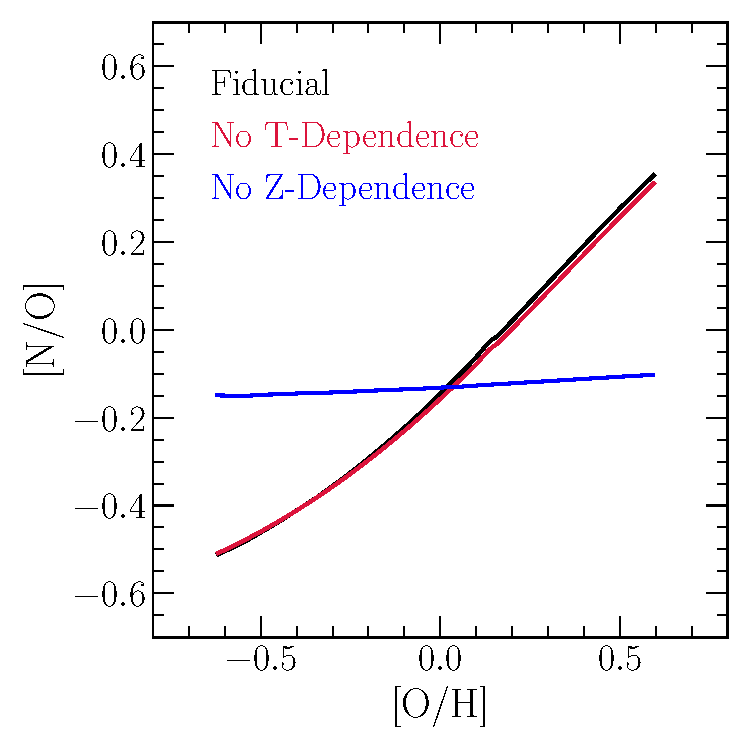
\includegraphics[scale = 0.63]{t_z_dep_comp.pdf}
\caption{
A comparison between our fiducial model with post-processing migration (black)
and variations with the time dependence (red) and metallicity dependence 
removed (blue).
To remove the time dependence, we pre-compute the AGB star yields of N from
13.2 Gyr old stellar populations as a function of metallicity as in the right
panel of Fig.~\ref{fig:ssp}, then incorporate this into the prompt CCSN yields
and set the delayed AGB star contribution to zero.
To remove the metallicity dependence, we evaluate the yields at our assumed
solar metallicity of~$Z = 0.014$ at all timesteps.
}
\label{fig:t_z_dep_comp}
\end{figure}

Despite predicting a different mass dependence for~\yagb{N}~(see Fig.
\ref{fig:agb_yield_models}), the renormalized~\cristallo~and~\ventura~yield
models both reproduce the slope of the~\ohno~relation reasonably well.
This is an indication that perhaps the metallicity dependence plays a much
more important role than the DTD in establishing this correlation.
To investigate this further, we consider two variants of our fiducial model:
one with the dependence on stellar age (or, equivalently, stellar mass)
removed from the enrichment rate calculations, and the other with the
metallicity dependence removed.
To make this comparison more straight-forward, we use the post-processing
migration model (see discussion in~\S~\ref{sec:multizone}).
\par
To remove the age dependence, we simply eject the AGB star yields alongside
the CCSN yield instantaneously after a single stellar population forms.
We pre-compute the N yields from all AGB stars associated with a 13.2 Gyr old
stellar population as a function of progenitor metallicity in a similar fashion
as in the right panel of Fig.~\ref{fig:ssp}; we use the linear yield model with
slope~$\xi = 9\times10^{-4}$ in this section.
Since~\vice~works from IMF-averaged CCSN yields assumed to be injected
instantaneously following a single stellar population's formation (see
discussion in~\S~\ref{sec:yields:ccsne}), we make use of the software's
capability to let the user specify functional forms for nucleosynthetic yields
and simply add this N yield to~\ycc{N}~and set~\yagb{N}~to zero.
In this model,~\ycc{N}~inherits a metallicity dependence from the AGB star
yields and has the exact shape as the curves in the right hand panel of
Fig.~\ref{fig:ssp}.
To remove the metallicity dependence, the procedure is much simpler: we simply
evaluate~\yagb{N}~at our assumed solar metallicity of~$Z = 0.014$ at all
timesteps regardless of that which is predicted for a stellar population.
In this variation, AGB star production still occurs on a DTD inherited from
the stellar mass-lifetime relation and the mass dependence of the linear yield
model.
\par
We illustrate these model predictions in Fig.~\ref{fig:t_z_dep_comp}.
The model with no age dependence is nearly identical to the~\ohno~relation
found in our fiducial model, while the model with no metallicity dependence
is considerably different.
This indicates that the metallicity dependence indeed plays a much larger role
than the DTD in establishing the overall shape of the~\ohno~relation.
This is rather unsurprising given the short characteristic timescales of N
production ($\sim$250 Myr, see the middle panel of Fig.~\ref{fig:ssp}).
Mathematically, there is little difference in the enrichment rates if all of a
stellar population's N is produced immediately as opposed to from a prompt,
sharply declining DTD.
The metallicity dependence, however, is paramount to the~\ohno~relation, which
is expected given the results in Fig.~\ref{fig:agb_yield_models} and consistent
with previous arguments that the increase in~\no~at high~\oh~is a consequence
of secondary N production~\citep{VilaCostas1993, vanZee1998, Henry1999,
PerezMontero2009, Berg2012, Pilyugin2012, Andrews2013, HaydenPawson2021}.
This however does indicate that our GCE model offers little if any
constraining power over the mass dependence of the AGB star yield of N.


\subsection{Comparison to Stellar Abundances in the Milky Way Disc}
\label{sec:results:vincenzo_comp}

% fig 8
\begin{figure}
\centering
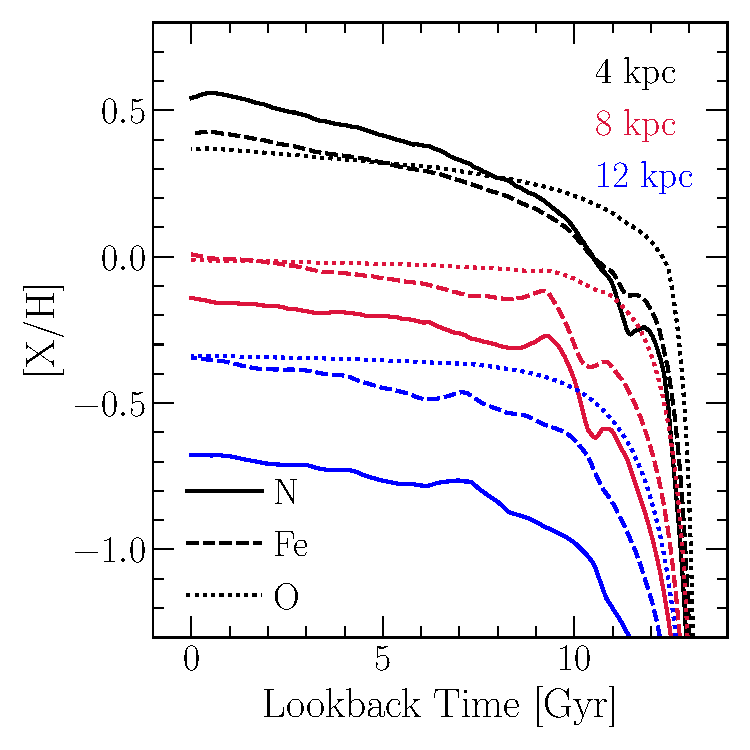
\includegraphics[scale = 0.63]{nh_feh_vs_lookback.pdf}
\caption{
\nh~(solid),~\feh~(dahsed), and~\oh~(dotted) in the gas-phase as a function of
lookback time in the fiducial model at~$\rgal = 4$ (black), 8 (red), and 12 kpc
(blue).
}
\label{fig:nh_feh_vs_lookback}
\end{figure}

% fig 9
\begin{figure*}
\centering
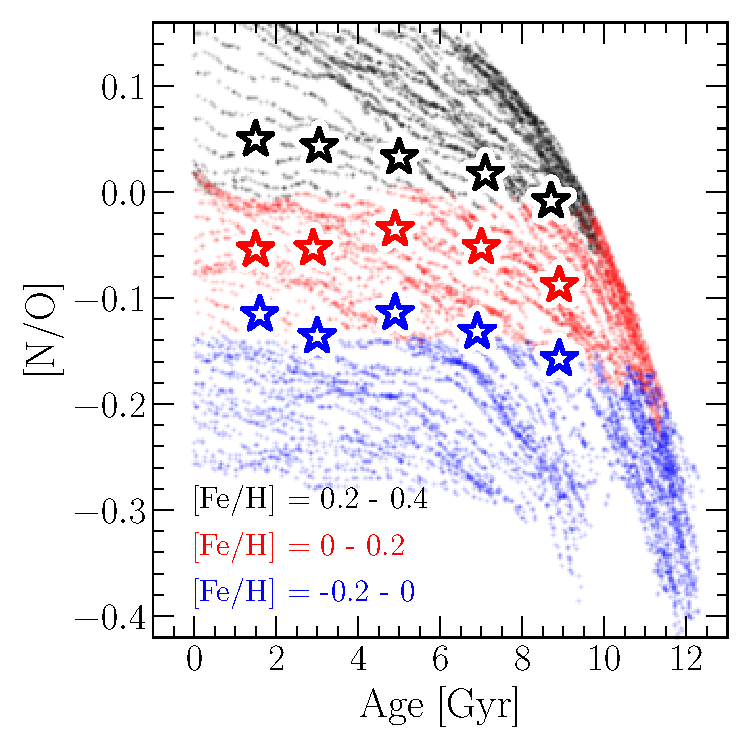
\includegraphics[scale = 0.55]{no_vs_age.pdf}
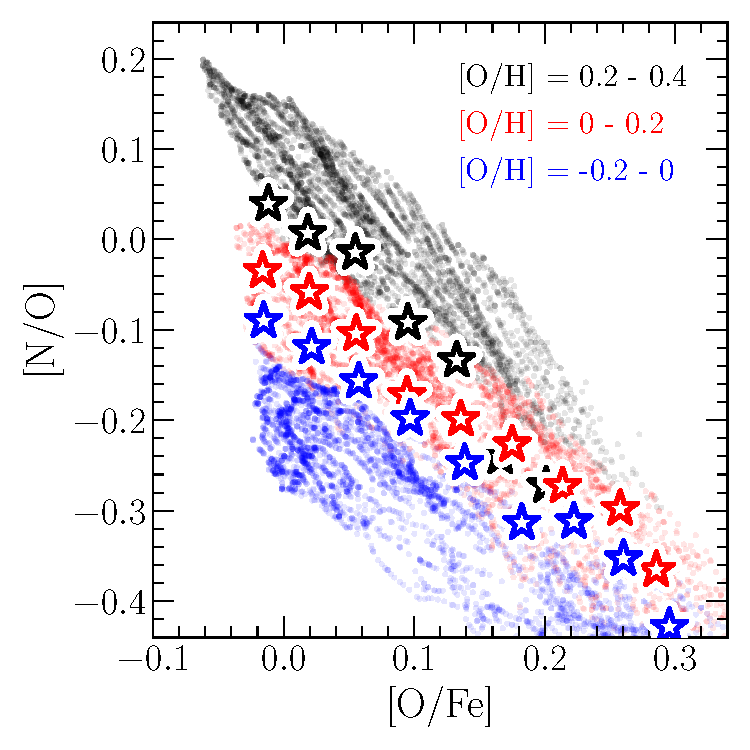
\includegraphics[scale = 0.55]{no_vs_ofe.pdf}
\caption{
\textbf{Left}:~\no~as a function of stellar age for 5000 stars randomly
sampled from our model stellar populations in three bins of~\feh~(coloured 
points).
Stars quantify the median trend in~\no~with age using N abundances corrected
for internal mixing processes reported by~\citet{Vincenzo2021} in the same
bins of~\feh.
\textbf{Right}: The same as the left panel, but instead showing~\no~as a
function of~\ofe~in bins of~\oh.
}
\label{fig:vincenzo_comp}
\end{figure*}

In Fig.~\ref{fig:nh_feh_vs_lookback}, we plot the evolution of N, O, and Fe
abundances in the gas phase at~$\rgal = 4$, 8, and 12 kpc in our fiducial model
with diffusion migration (see discussion in~\S~\ref{sec:multizone}).
\nh~is more correlated with~\feh~than~\oh~at all radii, and the relation
persists up to lookback times of~$\sim$10 Gyr.
This arises in part because N and Fe are both produced in significant
quantities by delayed enrichment sources while O is produced almost entirely on
short timescales by CCSNe (see discussion in~\S~\ref{sec:yields}).
Although the production timescale of N from single stellar populations is
short (see discussion in~\S~\ref{sec:yields:imf_agb}), metallicity dependent
yields require more abundant species such as O to be produced and reach an
equilibrium before N yields stabilize.
When many stellar populations are present, the bulk of the N production will
thus always follow the bulk production of more abundant species; this is 
qualitatively similar to what~\citet{Johnson2020} found regarding the
production timescales of Fe and strontium.
As a consequence of both its slight delay and its metallicity-dependent
yields, N reaches its equilibrium abundance on timescales similar to Fe rather
than O~\citep{Weinberg2017}.
Due to the prompt and metallicity independent nature of O enrichment,~\oh~is
near equilibrium as far back as~$\sim$10 Gyr ago while~\nh~and~\feh~are not.
This N-Fe correlation turns out to be important in understanding how these
model predictions compare to stellar abundances as we discuss below.
\par
Before comparing the predictions of GCE models to N abundances derived from
stellar spectra, it is essential to adjust the measurements for internal
processes known to alter the surface compositions of stars because GCE models
predict the birth abundances of stars.
After the CNO cycle has processed much of the C and O nuclei in a star's core
into~\Nfourteen~during its main sequence lifetime, this N-rich material is
mixed with the outer convective layers, increasing the N abundance in the
photosphere~\citep{Gilroy1989, Korn2007, Lind2008, Souto2018, Souto2019}.
\par
Using~\texttt{MESA} stellar evolution models~\citep{Paxton2011, Paxton2013,
Paxton2015, Paxton2018} with standard mixing prescriptions,~\citet{Vincenzo2021}
developed a recipe to approximate birth abundances of C, N and O and applied it
to a sample of APOGEE/Kepler red giants.
They found good agreement between the APOGEE abundances and the
\citet{Dopita2016} measurements, so our fiducial model's successful
reproduction of the~\citet{Dopita2016} trend is an indication that it should
also reproduce the~\ohno~relation for APOGEE disc stars.
Combining the~\citet{Vincenzo2021}~\no~ratios with the APOGEE stellar ages
taken from~\citet{Miglio2021}, we illustrate the~\no-age relation in bins
of~\feh~as predicted by our model in the left panel of Fig.
\ref{fig:vincenzo_comp}.
In good agreement with the observational measurements, the model predicts
the~\no-age relation to be relatively flat in bins of~\feh.
This arises as a consequence of the N-Fe correlation and the fast approach to
equilibrium in~\oh~as discussed above (see Fig.~\ref{fig:nh_feh_vs_lookback}).
A bin in~\feh~approximately corresponds to a bin in~\nh, and by extension a bin
in~\no~as well since~\oh~is nearly constant up to~$\sim$10 Gyr ago.
This is an important success of the model, because with uncorrected N
abundances,~\citet{Vincenzo2021} demonstrate that the~\no-age relation exhibits
a significant negative slope at fixed~\feh~(see their Fig. 7).
\par
In the right panel of Fig.~\ref{fig:vincenzo_comp}, we compare our model
predictions to the~\no-\ofe~relation at fixed~\oh~reported by
\citet{Vincenzo2021}.
The model correctly predicts a significant inverse relationship
between~\no~and~\ofe.
This is again a consequence of the N-Fe correlation demonstrated in
Fig.~\ref{fig:nh_feh_vs_lookback}:~\nh~increases with~\feh, so at
fixed~\oh,~\no~increases as~\ofe~decreases.
This is another important success of our model;~\citet{Vincenzo2021}
demonstrate that even when stellar N abundances are corrected for internal
mixing processes, the chemical dichotomy in~\no~between the high [$\alpha$/Fe]
and low [$\alpha$/Fe] disc populations persists (for discussion of the
Galaxy's two distinct chemical populations see, e.g.,~\citealp{Hayden2015,
Weinberg2019, Weinberg2021, Griffith2021b}).
Although the~\citet{Johnson2021} model does not reproduce the infamous
[$\alpha$/Fe] bimodality in detail (see discussion in their~\S~3.3), a future
iteration which does should also reproduce it for [N/O] based on these results.
\par
Quantitatively, our model slightly overpredicts~\no~in the lower metallicity
bins in both panels of Fig.~\ref{fig:vincenzo_comp}.
In general, our model occupies a noticeably wider range in~\no~than do the
\citet{Vincenzo2021} measurements at all ages and all~\ofe.
This could be a sign that the AGB star yields of N in our fiducial model scale
slightly too strongly with the total metallicity~$Z$.
Since our fiducial model assumes an exactly linear scaling of the N yield
with~$Z$ (see equation~\ref{eq:linear_yield}), this suggests that perhaps a
slightly sub-linear scaling would be more accurate, but only barely because
the discrepancies in Fig.~\ref{fig:vincenzo_comp} are at the~$\sim$0.1 dex
level.

\subsection{The Sources of Scatter in the~\ohno~Relation}
\label{sec:results:schaefer_comp}

\citet{Schaefer2020} demonstrate that intrinsic scatter in the
gas-phase~\ohno~relation is correlated with variations in the local SFE.
This is expected from simple GCE models: with slower star formation, more AGB
stars enrich the ISM by the time it reaches a given abundance, yielding a
higher~\no~at a given~\oh~\citep[e.g.][]{Molla2006, Vincenzo2016a}.
However,~\citet{Schaefer2020} did not rule out radial migration as another
potential source of scatter in this relation.
Our models, taking into account the effects of stellar migration on the
enrichment rates while allowing full control over the SFH and the SFE
through~\vice, are the ideal tool with which to address this question.
\par
To this end, we construct two variants of our fiducial model.
While the fiducial model specifies the SFH~\textit{a priori} and
lets~\vice~compute the infall history~$\dot{\Sigma}_\text{in}$, here we specify
the infall history as a function of radius and time.
As we will demonstrate below, the effects of dilution play an important role in
driving variations in the~\ohno~plane in these variants, and by specifying the
infall history we have more control over the amount of dilution.
Similar to other models discussed in this paper, we normalize
$\dot{\Sigma}_\text{in}$ such that a stellar mass consistent with that reported
by~\citet{Licquia2015} arises from the simulation.
All other evolutionary parameters are the same as in the~\citet{Johnson2021}
fiducial model.
\par
In the first variant, the SFE exhibits 50\% sinusoidal oscillations with time
over 2 Gyr periods:
\begin{equation}
\tau_\star(\rgal, t) = \tau_{\star,\text{J21}}(\rgal, t)
\left(1 + 0.5\sin\left(\frac{2\pi t}{2~\text{Gyr}}\right)\right).
\label{eq:sfe_var}
\end{equation}
The infall rate is constant in each ring with a value determined by normalizing
to the present day stellar mass and stellar surface density gradient of the
Milky Way.
Our choice of a 50\% amplitude is comparable to the observationally derived
scatter in molecular gas depletion times according to multiple measurement
methods (see Figs. 4 and 5 of~\citealp{Tacconi2018} and references therein).
Furthermore, variations in the SFE are of similar magnitude in~\hsim, the
galaxy from which our model's migration history is drawn.
In the second variant, the SFE is constant and the infall rate oscillates with
a 75\% amplitude about its mean value in the first variant:
\begin{equation}
\dot{\Sigma}_\text{in}(\rgal, t) = \langle\dot{\Sigma}_\text{in}\rangle
\left(1 + 0.75\sin\left(\frac{2\pi t}{2~\text{Gyr}}\right)\right).
\label{eq:ifr_var}
\end{equation}
The amplitude of 75\% is chosen such that the ensuing variability in the SFR is
of similar magnitude between the two models ($\sim$40\%).
We additionally run a model in which neither the accretion rate nor the SFE
oscillate, replacing the fiducial model used in previous sections.
Otherwise, the evolutionary differences beyond simple oscillations complicate
the comparison.

% fig 10
\begin{figure*}
\centering
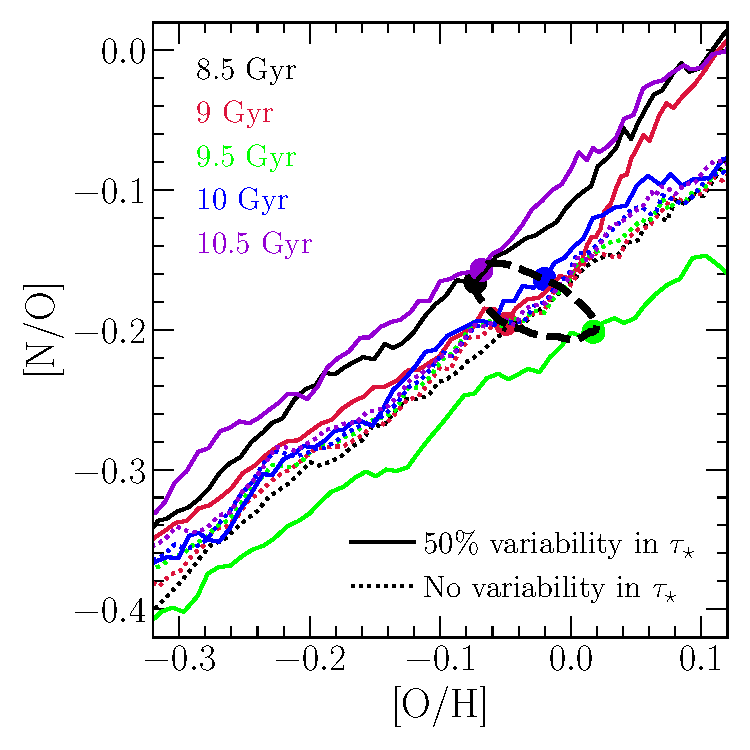
\includegraphics[scale = 0.44]{no_oh_sfevar.pdf}
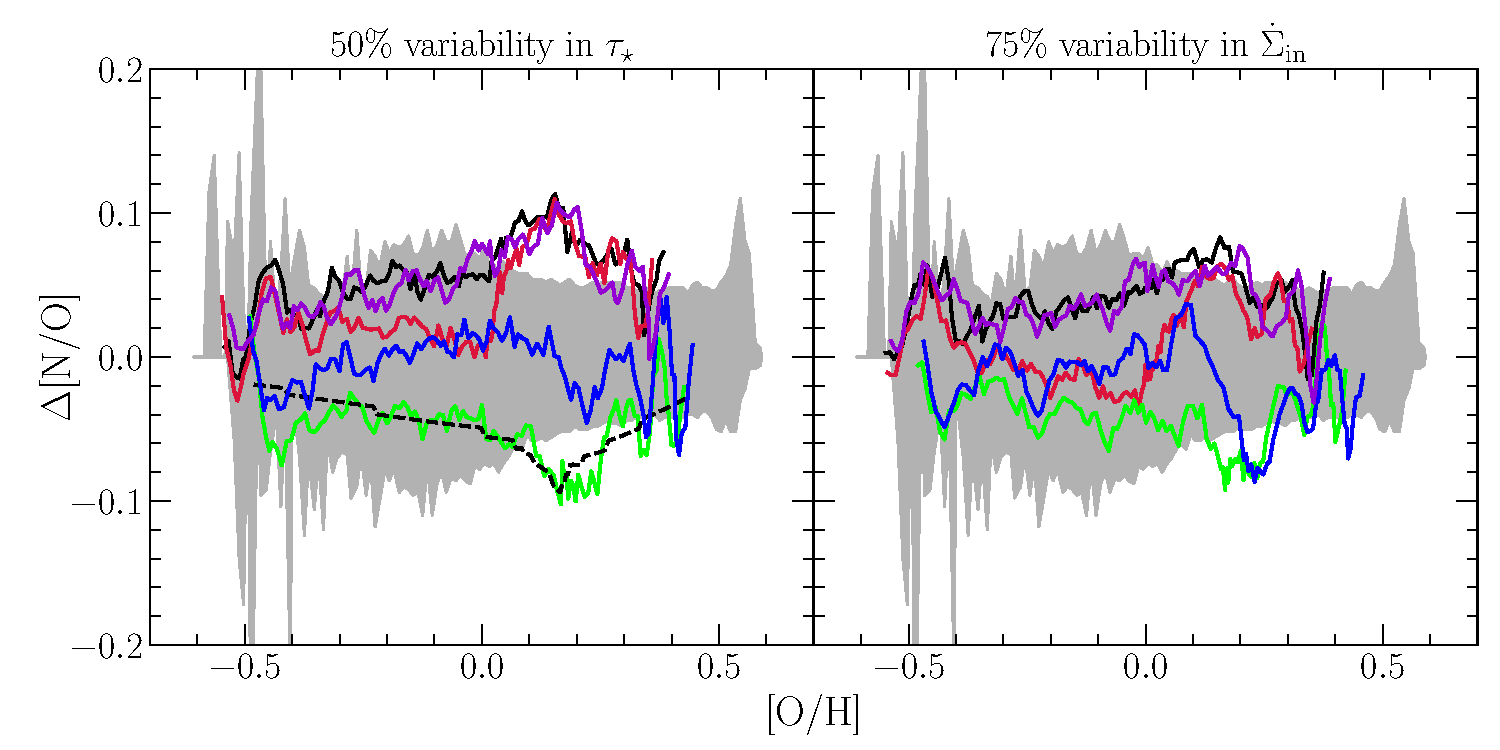
\includegraphics[scale = 0.47]{delta_no_schaefercomp.pdf}
\caption{
\textbf{Left}: One cycle of oscillations in the~\ohno~relation at
high~\oh~induced by 50\% sinusoidal variability in~$\tau_\star$ (solid coloured
lines).
Dotted lines show the~\ohno~relation at the same five snapshots in the fiducial
model with no variability in~$\tau_\star$ but still with diffusion migration
(see discussion in~\S~\ref{sec:multizone}).
The black dashed line shows the time evolution the abundances at~$\rgal = 8$
kpc, the approximate Galactocentric radius of the sun, with the times of each
of the five snapshots marked by a coloured point.
\textbf{Middle and Right}: For the same five snapshots in the left hand panel,
the deviation in~\no~at fixed~\oh~relative to the fiducial model for the case
with 50\% variability in~$\tau_\star$ (middle) and with 75\% variability
in~$\dot{\Sigma}_\star$ (right).
The shaded regions in both panels quantify the width of the [N/O] distribution
in~$10^{10.5} - 10^{11}~\msun$ galaxies in MaNGA taken from
\citet{Schaefer2020}.
In bins of~\oh, we place the median~\no~at~$\Delta\no = 0$, and the lower
(upper) envelope denotes the 16th (84th) percentile of the~\no~distribution.
}
\label{fig:schaefer_comp}
\end{figure*}

These variant models characterize evolutionary pathways in which star formation
is more episodic than previously explored.
% In the first, this arises out of internal processes at a constant accretion
% rate from the intergalactic medium, and may be caused by, e.g., star formation
% itself inducing a tug-of-war between heating and cooling processes.
% In the second, internal processes are suppressed and the episodic nature instead
% arises out of clumpy accretion events.
In a real galaxy, variability in the SFE and the SFR is likely non-sinusoidal
and not with constant amplitude.
A sample of galaxies will have different amplitudes and be seen at different
phases in their variability, and the impact of this on their N and O abundances
will present as intrinsic scatter in a sufficiently large sample.
By comparing models with and without reasonable amounts of variability in these
quantities while taking into account radial migration, we can nonetheless
assess which quantities impact abundances more strongly and are thus the more
likely causes of intrinsic scatter in the observed~\ohno~relation.
\par
In the left panel of Fig.~\ref{fig:schaefer_comp}, we plot the predicted
gas-phase~\ohno~relation for five snapshots covering one cycle of fluctuations
induced by variability in~$\tau_\star$ according to equation~\refp{eq:sfe_var}.
This model predicts a~$\sim$0.1 dex dynamic range in~\no~at fixed~\oh, whereas
the constant model with no variability in~$\tau_\star$ predicts the relation
to be nearly constant over this time interval.
This suggests that stellar migration, present in both the constant model and
this oscillatory variant, does not induce significant variability in
the~\ohno~plane; however, we demonstrate below that its effects are nonetheless
non-negligible.
The minimal impact of stellar migration traces back to the timescales of N
production from single stellar populations (see Fig.~\ref{fig:ssp} and
discussion in~\S~\ref{sec:yields:imf_agb}): with most N production occurring
within~$\sim$250 Myr of a stellar population's formation, most stars will not
migrate far from their birth radius by the time they produce most of their N,
and the resulting impact on abundances is small.
\par
The behavior in the~\ohno~plane predicted by the oscillatory SFE variant
is driven by the constant tug-of-war between dilution and re-enrichment
associated with oscillations in~$\tau_\star$.
When star formation quickens, O production increases in proportion.
The ISM abundance and consequently the N yields increase as well.
Because of the slight but nonetheless finite delay-time of its production by
AGB stars, the N enrichment rate lags slightly behind O.
\no~therefore decreases, and the ISM moves down and to the right in
the~\ohno~plane.
When star formation eventually slows, O production again follows suit.
The N enrichment rate, as before, lags slightly behind, and~\no~increases; the
ISM therefore moves up and to the left in the~\ohno~plane.
The result is an anti-clockwise loop, which we illustrate for the solar circle
with a black dashed line in the left panel of Fig.~\ref{fig:schaefer_comp}.
The effect is generally larger in~\oh~than in~\no~($\sim$0.1 dex versus
$\sim$0.05 dex in this example) because dilution affects
both~\oh~and~\nh~similarly.
The minimal increase in~\no~is thus a result of the small difference between N
and O production timescales.
In the model with oscillations in~$\dot{\Sigma}_\text{in}$, we find that
qualitatively similar processes drive the evolution in abundances, but there
are interesting differences in detail which we discuss below in the context of
scatter in the observed trend.
\par
In the middle and right panels of Fig.~\ref{fig:schaefer_comp}, we plot the
scatter in the gas-phase~\ohno~relation inferred observationally by
\citet{Schaefer2020}.
Using data from the MaNGA IFU survey~\citep{Bundy2015}, they measure N and O
abundances in 709,541 spaxels across 6,507 unique galaxies spanning
$10^9 - 10^{11}~\msun$ in stellar mass.
Since our model is appropriate for Milky Way mass galaxies, we focus our
comparison on the~$M_\star = 10^{10.5} - 10^{11}~\msun$ mass range
\citep{Licquia2015}, which cuts our sample sample to 197,787 individual N and O
measurements from the MaNGA IFU spaxels.
In narrow bins of~\oh, we then compute the 16th, 50th, and 84th percentiles of
the~\no~distribution.
Placing the median~\no~at~$\Delta\no = 0$, the shaded regions above and below
0 in Fig.~\ref{fig:schaefer_comp} denote the difference between 16th and 84th
percentiles of the distribution in each~\oh~bin.
\par
We compare both of our oscillatory variants to the width of the~\no~distribution
by over-plotting the difference in~\no~at fixed~\oh~between our oscillatory
models and their constant counterpart (i.e. the vertical offset between the
solid and dotted lines in the left panel, and the equivalent thereof for the
oscillatory~$\dot{\Sigma}_\text{in}$ model).
Both models produce offsets in~\no~at fixed~\oh~which, as discussed above,
arise as consequences of dilution, and the offsets are generally consistent
with the width of the relation derived observationally by~\citet{Schaefer2020}.
This supports their argument that variations in the local SFE can drive
intrinsic scatter in the~\ohno~relation, but the effects of stellar migration
are still non-negligible.
We demonstrate this by comparing the green solid and black dashed lines in the
middle panel, which denotes the same quantity from the oscillatory~$\tau_\star$
model with post-processing migration (see discussion in~\S~\ref{sec:multizone}).
As previously demonstrated in Fig.~\ref{fig:no_oh_timeevol} and discussed
in~\S~\ref{sec:results:fiducial}, stellar migration affects~\no~ratios with
an amplitude of~$\sim$0.05 dex, and this is apparent in
Fig.~\ref{fig:schaefer_comp} as well.
Although this is smaller than the impact of oscillations in either~$\tau_\star$
or~$\dot{\Sigma}_\text{in}$ ($\sim$0.1 dex), it is nonetheless significant
compared to the width of the~\citet{Schaefer2020} distributions, also at
the~$\lesssim$0.1 dex level; this suggests that stellar migration is a
non-negligible but subdominant source of scatter.
\par
In general, variability in~$\tau_\star$ impacts abundances more strongly than
variability in~$\dot{\Sigma}_\text{in}$.
Fig.~\ref{fig:schaefer_comp} shows similar changes in~\no~at fixed~\oh~in both
of our oscillatory variants, but it requires an amplitude of 75\% in accretion
rates to achieve the same~$\Delta\no$ as an amplitude of 50\% in the SFE.
This arises out of an abundance response which is much more~\textit{along}
the~\ohno~relation rather than~\textit{against} it as in the
oscillatory~$\tau_\star$ model (see the black dashed line in the left panel of
Fig.~\ref{fig:schaefer_comp}).
Both~\oh~and~\nh~vary with larger amplitudes in the variable infall model due to
episodes of enhanced and suppressed accretion, but the effects of dilution
on~\nh~are exacerbated by this in combination with metallicity dependent yields.
As a result,~\nh~varies with a larger amplitude than~\oh, whereas the opposite
is the case in the oscillatory~$\tau_\star$ model.
Consequently,~\no~increases rather than decreases with increasing~\oh, and
changes in~\no~at fixed~\oh~are smaller.
In the context of the observational results~\citep{Schaefer2020}, this suggests
that different~\no~ratios at fixed~\oh~are less likely to reflect changes in
the accretion rate than internal properties of the star forming ISM (e.g.
heating/cooling and pressure, which here get folded into~$\tau_\star$).

\end{document}

